\documentclass[10pt, oneside]{article}   	
\usepackage[left=25mm,top=25mm,right=25mm,bottom=25mm]{geometry}   
\usepackage[toc,page]{appendix}
\geometry{a4paper}
\usepackage{algorithm,algpseudocode}  
\usepackage{graphicx}
\usepackage{tikz}
\usepackage{pgfplots}					
\usepackage{amssymb}
\usepackage{amsmath}
\usepackage{gensymb}
\usepackage{multirow}
\usepackage{url}
\usepackage{titlesec}
\usepackage{subcaption}
\usepackage[export]{adjustbox}
\usepackage[parfill]{parskip}
\usepackage{cite}
\usepackage{hyperref}
\usepackage{array}
\usepackage{siunitx}
\usepackage{listings}
\usepackage{fixltx2e}
\usepackage{color}
\usepackage{diagbox}
\usepackage[parfill]{parskip}
\usepackage{pythonhighlight}
\setlength{\headsep}{5pt}
\graphicspath{ {images/} }
\lstset{
  basicstyle=\ttfamily,
  columns=fixed,
  fontadjust=true,
  basewidth=0.5em
}
\setcounter{topnumber}{3}
\setcounter{bottomnumber}{1}
\setcounter{totalnumber}{3}
\let\OLDthebibliography\thebibliography
\renewcommand\thebibliography[1]{
  \OLDthebibliography{#1}
  \setlength{\parskip}{0pt}
  \setlength{\itemsep}{1pt plus 0.5ex}
}
\renewcommand\thesection{\alph{section}}
\renewcommand\thesubsection{\thesection.\roman{subsection}}
\titleformat{\section}
{\normalfont\large\bfseries}{\thesection}{1em}{}
\titleformat{\subsection}
{\normalfont\normalsize\bfseries}{\thesubsection}{1em}{}
\title{\vspace{-1cm}Biomedical Information Processing (R214): Main Assignment}
\author{Chongyang Shi \emph{(cs940)}}
\date{\today}							
\begin{document}
\maketitle

For the main course assignment, I am undertaking the second practical option (\textbf{1.2}): \emph{extracting chemical-disease associations from the biological literature}.

\section{Improving the Conditional Random Fields named entity recognizer} \label{sec:a-crf-features}
\subsection{Ablating features from the original feature set} \label{subsec:ablating}

Based on the initial \emph{n}-gram feature set from the feature extraction script, the script was modified to ablate each feature in turn. To provide a better understanding of contributions from the offsets on surface form words, the entire word trigram was knocked out first, followed by just the -1/1 token offsets (leaving the unigram word behind). Other features knocked out in turn included the lemma, phonetic coding ($soundex$), part-of-speech, and chunk information in IOB2 notation, all of which were unigram by default, covering the current token only. The resulting precisions, recall rates, and $F_1$-scores from ablating each feature on the \emph{devel} dataset are presented separately in Figures \ref{fig:ablation1}, \ref{fig:ablation2}, and \ref{fig:ablation3}, with the corresponding performance of the original model as reference. Improved performance due to ablation are shown in \textbf{bold}.

\begin{figure}[h]
\begin{center}
\fontsize{9}{11}\selectfont
\begin{tabular}{|*{8}{c|}}\hline
\backslashbox{Class}{Ablated} & None & $word$ (all) & $word$ (-1/1) & $lemma$ & $soundex$ & $pos$ & $chunk$ \\ \hline
B-Chemical & 0.9178 & \textbf{0.9345} & \textbf{0.9409} & 0.9056 & 0.9015 & \textbf{0.9495} & \textbf{0.9210} \\ \hline
O                 & 0.9560 & 0.9471 & 0.9498 & 0.9540 & 0.9531 & 0.9499 & 0.9557 \\ \hline
B-Disease   & 0.8403 & 0.8242 & 0.8223 & \textbf{0.8418} & 0.8387 & \textbf{0.8412} & 0.8396 \\ \hline
I-Disease    & 0.7404 & 0.7152 & 0.7167 & \textbf{0.7467} & \textbf{0.7506} & \textbf{0.7631} & \textbf{0.7509} \\ \hline
I-Chemical  & 0.7556 & 0.6488 & 0.6745 & \textbf{0.7569} & \textbf{0.7612} & \textbf{0.7906} & \textbf{0.7682} \\ \hline
\textbf{Macro-average} & 0.8420 & 0.8142 & 0.8209 & 0.8410 & 0.8410 & \textbf{0.8589} &\textbf{ 0.8471} \\ \hline
\end{tabular}
\caption{\label{fig:ablation1} Resulting \textbf{precisions} on different named entity classes after ablating individual features from the original feature set.}
\end{center}
\end{figure}

\begin{figure}[h]
\begin{center}
\fontsize{9}{11}\selectfont
\begin{tabular}{|*{8}{c|}}\hline
\backslashbox{Class}{Ablated} & None & $word$ (all) & $word$ (-1/1) & $lemma$ & $soundex$ & $pos$ & $chunk$ \\ \hline
B-Chemical & 0.6664 & 0.5583 & 0.5955 & 0.6564 & 0.6520 & 0.5702 & 0.6652 \\ \hline
O                 & 0.9888 & 0.9888 & \textbf{0.9889} & 0.9888 & 0.9887 & \textbf{0.9908} & \textbf{0.9894} \\ \hline
B-Disease   & 0.6011 & 0.5514 & 0.5672 & 0.5669 & 0.5561 & 0.5806 & 0.5992 \\ \hline
I-Disease    & 0.6018 & 0.5530 & 0.5607 & 0.5993 & 0.5952 & \textbf{0.6029} & 0.5952 \\ \hline
I-Chemical  & 0.5961 & 0.5114 & 0.5275 & 0.5950 & 0.5910 & 0.5938 & \textbf{0.5990} \\ \hline
\textbf{Macro-average} & 0.6908 & 0.6326 & 0.6479 & 0.6813 & 0.6766 & 0.6677 & 0.6896 \\ \hline
\end{tabular}
\caption{\label{fig:ablation2} Resulting \textbf{recall rates} on different named entity classes after ablating individual features from the original feature set. }
\end{center}
\end{figure}

\begin{figure}[h]
\begin{center}
\fontsize{9}{11}\selectfont
\begin{tabular}{|*{8}{c|}}\hline
\backslashbox{Class}{Ablated} & None & $word$ (all) & $word$ (-1/1)& $lemma$ & $soundex$ & $pos$ & $chunk$ \\ \hline
B-Chemical & 0.7721 & 0.6992 & 0.7294 & 0.7611 & 0.7567 & 0.7125 & \textbf{0.7725} \\ \hline
O                 & 0.9721 & 0.9675 & 0.9690 & 0.9711 & 0.9706 & 0.9699 & \textbf{0.9723} \\ \hline
B-Disease   & 0.7008 & 0.6607 & 0.6713 & 0.6776 & 0.6687 & 0.6870 & 0.6993 \\ \hline
I-Disease    & 0.6640 & 0.6238 & 0.6292 & \textbf{0.6649} & 0.6639 & \textbf{0.6736} & \textbf{0.6641} \\ \hline
I-Chemical  & 0.6665 & 0.5720 & 0.5920 & 0.6662 & 0.6654 & \textbf{0.6782} & \textbf{0.6731} \\ \hline
\textbf{Macro-average} & 0.7551 & 0.7046 & 0.7182 & 0.7451 & 0.7451 & 0.7443 & \textbf{0.7562} \\ \hline
\end{tabular}
\caption{\label{fig:ablation3} Resulting \textbf{$F_1$-scores} on different named entity classes after ablating individual features from the original feature set.}
\end{center}
\end{figure}

Surprisingly, for chemicals at the start of entities (B-Chemicals), the precision (correct tags among those tagged) increased substantially when the entire surface form word trigram was knocked out. Ablating only the token offsets (-1/1) produced slightly higher precision than ablating the entire trigram. This is however at the cost of substantially reducing precisions for all other named entity classes, as well as reducing recall rates (correct tags among all relevant inputs that can be tagged) almost across the board. As B-chemicals already bear a fairly high precision (91.78\%), it is not advisable to ablate the surface forms, which would pull recall rates down into the 50\%-60\% range. 

Ablation of lemma (base word) and phonetic coding ($soundex$) features yielded minimal improvements to precisions on some named entity groups, while inflicting minimal reductions on others. Recall rates reduced by very small margins across the board. With generally negative outlooks of $F_1$-scores (combined measure of precision and recall) after knocking out either of these features, it is advisable not to ablate either.

Ablating part-of-speech produced the greatest precision improvements to most groups, but reduced the recall rate substantially for most named entity classes, especially for B-Chemicals. This is also reflected by the reduced $F_1$-scores. As part-of-speech provides local information around the observed token regarding the structure of the sentence, it is foreseeable that a lot more tokens would be mis-tagged without these information, resulting in the recall penalty. Therefore, it is not advisable to ablate the part-of-speech feature.

Finally, ablating the chunk information from the feature set improved the precision without significantly affecting the recall rate in most cases, resulting in improved $F_1$-scores for all named entity classes barring diseases within entities (I-Diseases, receiving a minor decrease). Therefore, it is advisable to ablate the chunk information from the feature set used.

Comparing vertically, precision and recall rates of terms outside entities (O) were high and only minimally affected by the ablation of any of the features. This is usually expected during entity recognition operations, due to the abundance of outside tokens between short named entities \cite{ratinov2009design}.

\subsection{Improvements to the base tagger}

After removing chunk information to improve performance of the base feature set as determined above, I first experimented with expanding the \emph{n}-gram feature set by extending unigram features into trigram features. After applying the favourable changes observed after the extensions, I examined the effects of adjusting several parameters of the L-BFGS training algorithm used in \emph{crfsuite}.

\subsubsection{Extension of unigram features}

During evaluations of word representation features used in entity recognition, Tang et al. \cite{tang2014evaluating} noted the benefits of utilising trigram features in word stemming. Drawing inspiration, I iteratively extended the unigram features of lemma, part-of-speech, and the phonetic coding ($soundex$) in the feature set. The order when extending the features was determined on the following basis: first extending lemma for its direction relation to word stemming; then part-of-speech with correlations between neighbouring words being considered important; and finally the phonetic coding being the one left from the original feature set. The resulting performance changes are shown in Figure \ref{fig:trigrams}.

\begin{figure}[h]
\begin{center}
\fontsize{9}{11}\selectfont
\begin{tabular}{|*{7}{c|}}\hline
\textbf{Expanded from unigram}  & \multicolumn{3}{c|}{None} & \multicolumn{3}{c|}{$lemma$}  \\ \hline 
\textbf{Entity Class} & Precision & Recall & $F_1$-score & Precision & Recall & $F_1$-score  \\ \hline
B-Chemical & 0.9210 & 0.6652 & 0.7725 & 0.9137 & 0.6695 & 0.7728 \\ \hline
O                 & 0.9557 & 0.9894 & 0.9723 & 0.9559 & 0.9890 & 0.9722\\ \hline
B-Disease   & 0.8396 & 0.5992 & 0.6993 & 0.8365 & 0.5992 & 0.6982 \\ \hline
I-Disease    & 0.7509 & 0.5952 & 0.6641 & 0.7519 & 0.6040 & 0.6699 \\ \hline
I-Chemical  & 0.7682 & 0.5990 & 0.6731 & 0.7820 & 0.6013 & 0.6798 \\ \hline
\textbf{Macro-average} & 0.8471 & 0.6896 & 0.7562 & 0.8480 & 0.6926 & 0.7586 \\ \hline \hline
\textbf{Expanded from unigram}  & \multicolumn{3}{c|}{$lemma$ + $pos$} & \multicolumn{3}{c|}{$lemma$ + $pos$ + $soundex$} \\ \hline 
\textbf{Entity Class} & Precision & Recall & $F_1$-score & Precision & Recall & $F_1$-score  \\ \hline
B-Chemical & 0.9077 & 0.6864 & 0.7817 & 0.9077 & 0.6875 & 0.7824 \\ \hline
O                 & 0.9574 & 0.9894 & 0.9731 & 0.9574 & 0.9894 & 0.9731 \\ \hline
B-Disease   & 0.8499 & 0.6162 & 0.7144 & 0.8477 & 0.6124 & 0.7111 \\ \hline
I-Disease    & 0.7819 & 0.6103 & 0.6855 & 0.7795 & 0.6110 & 0.6850 \\ \hline
I-Chemical  & 0.7884 & 0.6138 & 0.6903 & 0.8010 & 0.6241 & 0.7016 \\ \hline
\textbf{Macro-average} & 0.8570 & 0.7032 & 0.7690 & 0.8587 & 0.7049 & 0.7706 \\ \hline
\end{tabular}
\caption{\label{fig:trigrams} Resulting tagging performance on the \emph{devel} dataset after incrementally extending unigram features into trigram features. ``None'' represents the original feature set with $chunk$ ablated.}
\end{center}
\end{figure}

While the precision of B-Chemical tagging continued to follow the declining trend as discussed in \ref{subsec:ablating} (although not as severe as in feature ablation), expanding unigram features of lemma, part-of-speech, and the phonetic coding into trigrams all resulted in improved or largely unchanged precisions, recall rates, and $F_1$-scores. Precision improvements were most significant after the expansions of lemma and phonetic coding on chemicals within entities (I-Chemicals), displaying the considerable influence of nearby phonetic features on chemical entity recognition accuracy. The strongest improvements in recall and the $F_1$-score came from expanding part-of-speech, again demonstrating the importance of an extended semantic scope. While precisions of some named entities took a small hit when the phonetic coding ($soundex$) was added, the improved macro-average precision as well as generally improved recall rates and $F_1$-scores backed my choice of retaining all three extensions of unigrams into trigrams in the feature set.

\subsubsection{Adjustment of training parameters}

The L-BFGS training algorithm used in entity recognition performs L2 regularization, which is usually more efficient than L1 \cite{cortes20092}, with a regularization parameter ($c2$) controlling the trade-offs between bias and overfitting. Various values of $c2$ around the default $c2 = 1$ were tested, with broadly similar trends in precision, recall, and $F_1$-score on individual named entities. Therefore, only the macro-averages from tagging the \emph{devel} dataset with a model trained on different values of $c2$ are plotted in Figure \ref{fig:c2}.

\begin{figure}[h]
\begin{center}
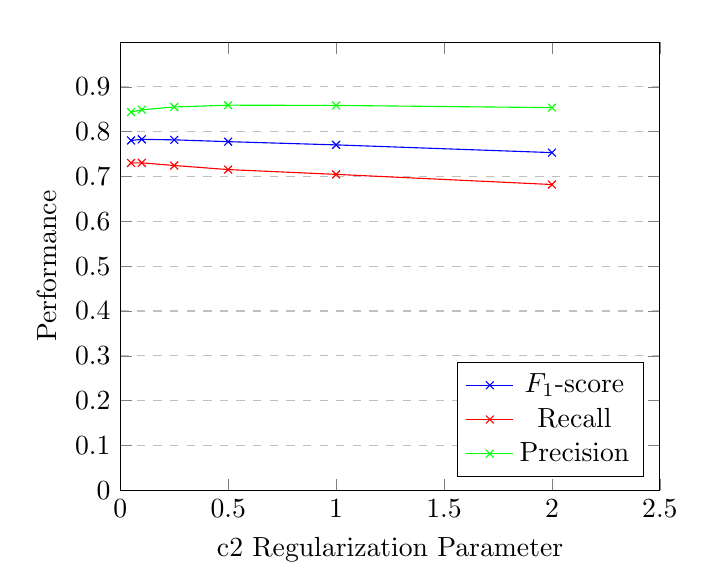
\begin{tikzpicture}
\begin{axis}[
    xlabel={c2 Regularization Parameter},
    ylabel={Performance},
    xmin=0, xmax=2.5,
    ymin=0, ymax=1.0,
    xtick={0, 0.5, ..., 2.5},
    ytick={0, 0.1, ..., 1.0},
    legend pos=south east,
    ymajorgrids=true,
    grid style=dashed,
]
 
\addplot[
color=blue,
mark=x,
]
coordinates {
(0.05,0.780505)(0.1,0.782937)(0.25,0.781873)(0.5,0.777822)(1.0,0.770645)(2.0,0.753415)
};
\addplot[
color=red,
mark=x,
]
coordinates {
(0.05,0.730290)(0.1,0.730579)(0.25,0.724635)(0.5,0.715561)(1.0,0.704877)(2.0,0.682223)
};
\addplot[
color=green,
mark=x,
]
coordinates {
(0.05,0.843873)(0.1,0.848921)(0.25,0.855177)(0.5,0.859233)(1.0,0.858653)(2.0,0.853710)
};
\legend{$F_1$-score,Recall,Precision}
\end{axis}
\end{tikzpicture}
\caption{\label{fig:c2} Resulting tagging performance on the \emph{devel} dataset with models trained on different c2 values.}
\end{center}
\end{figure}

A reduced $c2$ parameter resulted in longer training, but also generally improved recall and the overall $F_1$-score. Considering the adverse effects of extended training time and reduced precision due to increased overfitting, as well as diminishing gains in recall, $c2=0.25$ was chosen as the final $c2$ value.

L-BFGS also supports different line search algorithms, which when alternated yielded roughly the same training speed and performance for all named entity classes, as shown in Figure \ref{fig:linesearch}. Therefore the default More and Thuente's method was retained as the line search algorithm.

\begin{figure}[h]
\begin{center}
\fontsize{9}{11}\selectfont
\begin{tabular}{|*{10}{c|}}\hline
\textbf{Line Search}  & \multicolumn{3}{c|}{$MoreThuente$} & \multicolumn{3}{c|}{$Backtracking$} & \multicolumn{3}{c|}{$StrongBacktracking$}  \\ \hline 
\textbf{Entity Class} & Precision & Recall & $F_1$-score & Precision & Recall & $F_1$-score & Precision & Recall & $F_1$-score \\ \hline
B-Chemical & 0.9223 & 0.6972 & 0.7941 & 0.9223 & 0.6972 & 0.7941 & 0.9223 & 0.6972 & 0.7941 \\ \hline
O                 & 0.9609 & 0.9884 & 0.9745 & 0.9609 & 0.9884 & 0.9744 & 0.9609 & 0.9884 & 0.9744 \\ \hline
B-Disease   & 0.8363 & 0.6671 & 0.7422 & 0.8353 & 0.6656 & 0.7409 & 0.8352 & 0.6661 & 0.7411 \\ \hline
I-Disease    & 0.7515 & 0.6338 & 0.6876 & 0.7520 & 0.6330 & 0.6874 & 0.7520 & 0.6330 & 0.6874 \\ \hline
I-Chemical  & 0.8048 & 0.6367 & 0.7110 & 0.8048 & 0.6367 & 0.7110 & 0.8048 & 0.6367 & 0.7110 \\ \hline
\textbf{Macro-average} & 0.8552 & 0.7246 & 0.7819 & 0.8550 & 0.7242 & 0.7816 & 0.8550 & 0.7243 & 0.7816 \\ \hline
\end{tabular}
\caption{\label{fig:linesearch} Resulting tagging performance on the \emph{devel} dataset with different line search algorithms: More and Thuente's method, backtracking method with regular Wolfe condition, and backtracking method with strong Wolfe condition.}
\end{center}
\end{figure}

\subsection{Evaluating the improved model on the test set}

To summarise, the changes made on the original entity recognition model include the ablation of chunk information from the feature set during feature extraction; extensions of lemma, part-of-speech, and phonetic coding ($soundex$) features from unigrams into trigrams (covering features of tokens before and after the current one); as well as adjusting L-BFGS' $c2$ regularization parameter to 0.25. A comparison between the improved model and the original model when tagging the \emph{test} dataset is shown in Figure \ref{fig:improved-compare}.

\begin{figure}[h]
\begin{center}
\fontsize{9}{11}\selectfont
\begin{tabular}{|*{7}{c|}|c|}\hline
\textbf{Model}  & \multicolumn{3}{c|}{\textbf{Improved}} & \multicolumn{3}{c||}{\textbf{Original}} & \emph{Change} \\ \hline 
\textbf{Entity Class} & Precision & Recall & $F_1$-score & Precision & Recall & $F_1$-score & $F_1$-score \\ \hline
B-Chemical & 0.9168 & 0.6771 & 0.7789 & 0.9085 & 0.6457 & 0.7549 & +3.18\% \\ \hline
O                 & 0.9619 & 0.9890 & 0.9753 & 0.9576 & 0.9882 & 0.9726 & +0.28\% \\ \hline
B-Disease   & 0.8218 & 0.6514 & 0.7268 & 0.8217 & 0.5895 & 0.6865 & +5.87\% \\ \hline
I-Disease    & 0.7522 & 0.6434 & 0.6936 & 0.7311 & 0.6178 & 0.6697 & +3.57\% \\ \hline
I-Chemical  & 0.7998 & 0.6087 & 0.6913 & 0.7438 & 0.6081 & 0.6691 & +3.32\% \\ \hline
\textbf{Macro-average} & 0.8505 & 0.7139 & 0.7732 & 0.8325 & 0.6899 & 0.7506 & +3.01\% \\ \hline
\end{tabular}
\caption{\label{fig:improved-compare} Performance comparison between the improved entity recognition model and the original model on tagging the \emph{test} dataset.}
\end{center}
\end{figure}

Feature set and parameter changes resulted in a model with improved precision and recall across the board. As the combined measure of precision and recall, changes in $F_1$-scores are also shown on the right of Figure \ref{fig:improved-compare}. Terms outside entities (O's) with already high precision and recall received the least improvement, while disease terms at the start of entities (B-Diseases) benefited the most from the improved model. Greater than 3\% of improvements were observed for all other named entity classes and the macro-average. Based on these results from tagging the unseen \emph{test} input dataset, I believe it is reasonable to conclude that for entity recognition of environmental and disease concepts, the improved model is superior to the original model.

\section{Grounding named entities through approximate string matching} \label{sec:grounding}

The MESH concept dictionary contains terms from two classes of entities: chemicals and diseases. For the lemma of each tagged token within a chemical or disease entity, all possible choices of the relevant class from the MESH dictionary were supplied to an approximate string matching process facilitated by the \verb|fuzzywuzzy| \cite{fuzzywuzzy} library. With a na\"ive approach allowing the simplest implementation, the tokens were grounded individually. (In the examples presented below, \verb|**| will be used to annotate grounded terms in the sentence, with reference numbers pointing to entity names grounded from the dictionary).

Unfortunately, this na\"ive approach appeared to be clearly inadequate, as multi-token entities were not reassembled:

\begin{lstlisting}[breaklines]
**Urine**{1} **N**{2} **-**{3} **acetyl**{4} **-**{5} **beta**{6} **-**{7} **D**{8} **-**{9} **glucosaminidase**{10} - - a marker of **tubular**{11} **damage**{12} ?
{1} purine (Score: 91)
{2} alanine (Score: 90)
{3} 11-deoxycortisol (Score: 0)
{4} 2-acetylaminofluorene (Score: 90)
{5} 11-deoxycortisol (Score: 0)
{6} 17beta-estradiol (Score: 90)
{7} 11-deoxycortisol (Score: 0)
{8} 1,2-DMH (Score: 90)
{9} 11-deoxycortisol (Score: 0)
{10} AMI (Score: 90)
{11} acute tubular necrosis (Score: 90)
{12} axonal damage (Score: 90)
\end{lstlisting}

The first ten terms extracted from the above sentence were designated as being outside a named entity class (``O'') by the reference labels, but mis-recognised by the entity recognition model as a chemical spanning across multiple terms (in fact, the original term is an enzyme, which can be counted as a chemical but not included in the dictionary). The resulting attempt to match the fragmented components individually produced a long list of poorly matched entities. Similarly, the fragmentation of ``tabular'' and ``damage'' resulted in them being individually matched with separate, irrelevant entities from the dictionary.

These two errors highlighted the need of reassembling neighbouring tokens belonging to the same entity before attempting grounding. Therefore, \textbf{the grounding process was modified to first reassemble these neighbouring terms together} (e.g. from ``... + $O$ + $B-Chemical$ + $I-Chemical$ + $I-Chemical$ +  $O$ + ...'' to ``... + $O$ + $Chemical$ +  $O$ + ...'') before matching the assembled term with the best approximation in the dictionary. The previous grounded example is now:

\begin{lstlisting}[breaklines]
**Urine N - acetyl - beta - D - glucosaminidase ** {1} - - a marker of **tubular damage ** {2} ? 
{1} 9-[[2-methoxy-4-[(methylsulphonyl)amino]phenyl]amino] -N,5-dimethyl- 4-acridinecarboxamide (Score: 86)
{2} acute tubular necrosis (Score: 86)
\end{lstlisting}

While the enzyme is still not matched by an appropriate entity from the dictionary (as it is not included), with reassembly applied, ``acute tubular necrosis'' is now a very good biomedical description of ``tubular damage'' in the original text. To further resolve the lack of dictionary coverage over complex chemical constructs, concept associations generated from co-occurrences of functional groups \cite{tsuruoka2008facta} could aid the grounding system in finding the best-matching entity efficiently.

Overall, the grounding method with entity reassembly worked fairly well, such as on the following sentence:

\begin{lstlisting}[breaklines]
BACKGROUND : **Calcitriol ** {1} therapy suppresses serum levels of parathyroid hormone ( PTH ) in patients with **renal failure ** {2} but has several drawbacks , including **hypercalcemia ** {3} and / or marked suppression of bone turnover , which may lead to adynamic bone disease . 
{1} Ca (Score: 90)
{2} renal failure (Score: 100)
{3} hypercalcemia (Score: 100)
\end{lstlisting}

While Calcitriol does not exist in the MESH dictionary, it does increase the body's intake of its closest match in the dictionary -- Calcium (Ca). Although this is mostly a lucky match due to the lack of a less relevant term with a shorter edit distance, similar processes of inferring terms through biomedical relations have already been applied on other dictionaries to improve grounding performance, such as inferring through contrastive information between proteins \cite{kim2005biocontrasts}. More systematically, machine learning-based inference systems trained on biomedical databases (e.g. gene ontology) can be used to effectively construct knowledgebase from unstructured biomedical information \cite{shin2015incremental}. 

In the above example, ``renal failure'' was also correctly matched with the corresponding term in the dictionary after entity reassembly. Other issues do however persist after the reassembly modification, such as the inability to match uncommon acronyms with their full base words:

\begin{lstlisting}[breaklines]
(Simple acronyms, easy matching)
CBA / **Ca ** {1} male mice started on **AZT ** {2} 0 . 75 mg / ml **H2O ** {3} at 84 days of age and kept on it for 687 days when dosage reduced to 0 . 5 mg / ml **H2O ** {4} for a group , another group removed from **AZT ** {5} to see recovery , and third group remained on 0 . 75 mg . 
{1} Ca (Score: 100)
{2} AZT (Score: 100)
{3} H2O (Score: 100)
{4} H2O (Score: 100)
{5} AZT (Score: 100)

(Complex, lesser-known acronyms, hard matching)
RESULTS : In Nx dogs , **OCT ** {1} significantly decreased serum PTH levels soon after the induction of **renal insufficiency ** {2} . 
{1} methoctramine (Score: 90)
{2} renal insufficiency (Score: 100)
\end{lstlisting}

From the original literature \cite{monier199922}, ``OCT'' refers to Oxacalcitriol, which is not present in the dictionary, causing ``OCT'' to be interpreted as methoctramine. However, even if Oxacalcitriol was in the dictionary, it is unlikely that crude approximate string matching would have found Oxacalcitriol from ``OCT'' with a long edit distance involved, when scrambled with confusing terms such as ``OCD'' already in the dictionary. It is possible, however, to resolve most acronyms into canonical forms with static or dynamic rules generated from ontology knowledge \cite{naderi2011organismtagger}.

Finally, common sections of biomedical composite words and multi-word nouns can cause incorrect groundings when a direct match with the dictionary vocabulary is not possible. For example:

\begin{lstlisting}[breaklines]
Histological examination on 9 of 10 mice with such **thrombocytopenia ** {1} showed changes compatible with **myelodysplastic syndrome ** {2} ( **MDS ** {3} ) . 
{1} thrombocytopenia (Score: 100)
{2} Fanconi syndrome (Score: 86)
{3} DES (Score: 67)
\end{lstlisting}

Myelodysplastic syndromes are associated with bone marrows, while Fanconi syndrome describes kidney conditions. With vastly different natures of conditions, results from this grounding attempt were erroneous. Methods to better distinguish semantic compositions of compound words (known as ``compound bracketing'') with unsupervised probabilistic models \cite{pecina2010lexical}, as well as CRF post-processing and lexicon/dictionary-supported normalization \cite{lee2016audis} have been developed to improve accuracy when grounding compound words and multi-word nouns.

In summary, a better grounding system may have the following features:
\begin{itemize}
	\item Functional group associations that can be queried efficiently \cite{tsuruoka2008facta} are used to find best-matching entities of complex chemical constructs if a direct match in vocabulary is not possible;
	\item For sources containing unstructured biomedical information, databases storing relational information \cite{kim2005biocontrasts} between entities are used to train inference agents \cite{shin2015incremental} to better resolve terms without a direct match;
	\item To resolve unfamiliar acronyms not present in the dictionary, rules generated from ontology databases are applied to resolve the acronyms into canonical forms \cite{naderi2011organismtagger}, which are more likely to encounter good matches during grounding;
	\item Unsupervised probabilistic models \cite{pecina2010lexical} and CRF-based normalization algorithms \cite{lee2016audis} are used to improve accuracy when grounding composite terms.
\end{itemize}

\section{Identifying associations between disease and chemical mentions}

The full abstract collection of PubMed texts on chemically induced disorders numbered 301,084,933 lines, with words already pre-processed into a format identical to those used as source in Section \ref{sec:a-crf-features}. With referencing named entity classes unavailable (defaulting to outside entities), the improved entity recognition model trained in Section \ref{sec:a-crf-features} was used to perform entity recognition on all 301,084,933 lemmas of surface form words from 10,573,978 sentences. Tags generated through entity recognition were then cross-referenced with the original surface words and their lemmas for grounding, the process of which was conducted in parallelised batches to reduce memory footprint. 

\subsection{Simple co-occurrence counts} \label{subsec:simple-co}

With grounded entities grouped by the sentences they originated from, duplications of entities within the same sentence were removed, with the assumption that multiple mentions of a noun entity in the same sentence are primarily for clarity rather than emphasis \cite{clark1979search}. Grounded entities in the sentence were then sorted into a consistent alphanumeric order to preserve consistent ordering of co-mention pairs. Mentioning of a unique entity within a sentence was recorded globally as an occurrence of that entity. 

All possible in-order combinations of grounded entities were then generated (length of 2 only), forming pairs of entities within the same sentence. Based on the context of the study, an additional filter was placed so that only co-mention pairs of a chemical and a disease will be recorded. Implementations of these pre-processing steps can be found in Figure \ref{fig:preprocessing} within Appendix \ref{sec:implementations}.

The ten most common grounded entities and the pairs thereof from the PubMed abstract texts are shown in Figure \ref{fig:popular-individuals} and Figure \ref{fig:popular-pairs}.

\begin{figure}[h]
\begin{center}
\fontsize{9}{11}\selectfont
\begin{tabular}{|*{3}{c|}p{2cm}||*{3}{c|}p{2cm}|}\hline
\multicolumn{4}{|c||}{\textbf{Chemicals}} & \multicolumn{4}{c|}{\textbf{Diseases}} \\ \hline 
Count & Probability & MESH ID & Name & Count & Probability & MESH ID & Name \\ \hline 
248227 & 0.045\% & D006859 & H & 166561 & 0.030\% & D009369 & tumour \\ \hline 
135662 & 0.024\% & D009569 & NO & 155455 & 0.028\% & D004714 & endometrial hyperplasia or cancer \\ \hline 
102140 & 0.018\% & D008694 & METH & 128998 & 0.023\% & D064420 & Toxicity \\ \hline 
79642 & 0.014\% & C034818 & methyl 6,7-dimethoxy-4-ethyl-B-carboline-3-carboxylate & 60568 & 0.011\% & D020511 & disorder of neuromuscular transmission \\ \hline 
78439 & 0.014\% & C066430 & 3-aminopropyl-diethoxy-methyl-phosphinic acid & 58780 & 0.011\% & D007239 & infections \\ \hline 
70656 & 0.013\% & C025136 & phenylacetic acid & 54426 & 0.010\% & D047508 & massive hepatocellular necrosis \\ \hline 
68107 & 0.012\% & D004298 & Dopamine & 51521& 0.009\% & D003643 & deaths \\ \hline 
65758 & 0.012\% & D018698 & glutamine & 44556 & 0.008\% & D012140 & respiratory and cardiovascular depression \\ \hline 
63797 & 0.011\% & D005947 & glucose & 40723 & 0.007\% & D031901 & gestational trophoblastic disease \\ \hline 
62878 & 0.011\% & D002118 & Calcium & 38994 & 0.007\% & D008103  & cirrhosis of the liver \\ \hline 
\end{tabular}
\caption{\label{fig:popular-individuals} The top ten most commonly mentioned chemical and disease entities by appearance in number of sentences.}
\end{center}
\end{figure}

\begin{figure}[h]
\begin{center}
\fontsize{9}{11}\selectfont
\begin{tabular}{|*{6}{c|}}\hline
\multicolumn{2}{|c|}{\textbf{Association}} & \multicolumn{2}{c|}{\textbf{Chemical}} & \multicolumn{2}{c|}{\textbf{Disease}} \\ \hline 
Count & Probability & MESH ID & Name & MESH ID & Name \\ \hline 
6425 & 0.00116\% & D003404 & creatinine & D009369 & tumour \\ \hline
5860 & 0.00105\% & D003404 & creatinine & D047508 & massive hepatocellular necrosis \\ \hline
5180 & 0.00093\% & D006859 & H & D020511 & disorder of neuromuscular transmission \\ \hline
3995 & 0.00072\% & D004967 & estrogen & D004714 & endometrial hyperplasia or cancer \\ \hline
3850 & 0.00069\% & D005472 & 5-FU & D004714 & endometrial hyperplasia or cancer \\ \hline
3259 & 0.00059\% & D006859 & H & D012140 & respiratory and cardiovascular depression \\ \hline
3162 & 0.00057\% & D002945 & cisplatinum & D004714 & endometrial hyperplasia or cancer \\ \hline
3112 & 0.00056\% & D004317 & Doxorubicin & D004714 & endometrial hyperplasia or cancer \\ \hline
2986 & 0.00054\% & D006859 & H & D004714 & endometrial hyperplasia or cancer \\ \hline
2902 & 0.00052\% & D002945 & cisplatinum & D009369 & tumour \\ \hline
\end{tabular}
\caption{\label{fig:popular-pairs} The top ten most common associations of chemical and disease entities by appearance in number of sentences.}
\end{center}
\end{figure}

It was expected that, by the sole criterion of number of occurrences, chemicals and syndromes of conditions commonly involved in the studies of environments and diseases will occupy a significant proportions of the top tens. This was confirmed in Figure \ref{fig:popular-individuals} with the presence of hydrogen, nitrogen oxide, calcium, as well as ``tumour'', ``infections'' and ``deaths''. These concepts alone do not confer a significant amount of useful information about chemically induced disorders. Entities related to more specific concepts do however exist, such as two chemicals (C034818, C066430) associated with modulation of GABAA receptors, which affect anxiety-related mental states, suggesting the relative prominence of GABAA-related studies among the abstract texts. Diseases concerning different organs among the top ten are also good indicators of common lesions involved in the studies.

Apart from the suggested potential links between creatinine, cisplatinum (Cisplatin), and tumours; most of the top co-mentions based on simple co-occurrence counts in Figure \ref{fig:popular-pairs} were associated with a single class of diseases -- endometrial hyperplasia or cancer. This signals a key limitation in ranking associations based on simple co-occurrence counts: source texts with imbalanced compositions of study can make broad observations of associations between chemicals and diseases difficult. Once again the three associations between hydrogen and diseases provide very little useful information, as hydrogen is an almost-universal component of organic molecules. 

To improve the effectiveness of co-occurrence count-based rankings, it may be possible to take ideas from object categorisation techniques by considering relative locations (which are locations of grounded entities in sentences in text mining)\cite{galleguillos2008object}, or to borrow from machine translation techniques and apply arithmetic and geometric mean functions to co-occurrence counts from an imbalanced corpus \cite{zhu2014improving}. Ultimately however, the aforementioned issues prompt more sophisticated statistical measures to be deployed, in order to better identify the links between environmental chemicals and diseases.

\subsection{Statistical measures}

For the purpose of calculating occurrence probabilities, all sentences with any mention of a chemical or disease are counted into the total, even if a pair of chemical and disease cannot be established within the sentence. This is to maintain probability consistency between chemical occurrences and disease occurrences. In addition to occurrences of individual and pairs of entities, four statistical measure were considered: Pointwise Mutual Information (PMI), Normalized Pointwise Mutual Information (NPMI), the Jaccard coefficient/index, and Symmetric Conditional Probability (SCP). With occurrences of pairs of chemical and disease entities recorded in dictionaries indexed by 2-tuples of IDs, calculations of these statistical co-occurrence metrics for pairs of entities were straightforward through dictionary comprehensions, as shown in Figure \ref{fig:stats-calc} within Appendix \ref{sec:implementations}. Top ten associations as measured by these metrics are shown in Figures \ref{fig:pmi}, \ref{fig:npmi}, \ref{fig:jaccard}, and \ref{fig:scp} respectively. Logarithms with base 2 were used for all logarithmic calculations.

\begin{figure}[h]
\begin{center}
\fontsize{9}{11}\selectfont
\begin{tabular}{|*{2}{c|}p{4.5cm}|c|p{4.5cm}|}\hline
 \multirow{2}{*}{\textbf{PMI}} & \multicolumn{2}{c|}{\textbf{Chemical}} & \multicolumn{2}{c|}{\textbf{Disease}} \\ \cline{2-5}
 & MESH ID   & Name                      & MESH ID   & Name                         \\ \hline
 8.95518 & C476217   & cinacalcet HCl            & D006961   & hyperparathyroidism          \\ \hline
 8.72841 & D005702   & Galanthamine hydrobromide & D014826   & vocal fold palsy             \\ \hline
 8.35901 & D013390   & Suxamethonium chloride    & D005207   & Fasciculations               \\ \hline
 8.35375 & D011441   & Propylthiouracil          & D006980   & hyperthyroidism              \\ \hline
 8.31867 & D013390   & Suxamethonium chloride    & D012019   & reflex sympathetic dystrophy \\ \hline
 8.31393 & C031942   & argatroban                & D013684   & telangiectasis               \\ \hline
 8.16299 & D005013   & ethosuximide              & D004832   & absence seizures             \\ \hline
 8.07865 & D008972   & molindone                 & D002819   & Choreoathetoid movements     \\ \hline
 7.99780 & D007464   & clioquinol                & C538178   & acrodermatitis enteropathica \\ \hline
 7.83060 & D004025   & dicyclomine               & D004211   & intravascular coagulation    \\ \hline
\end{tabular}
\caption{\label{fig:pmi} The top ten associations of chemical and disease entities as measured by Pointwise Mutual Information (PMI).}
\end{center}
\end{figure}

With mutual dependence between pairs of chemicals and diseases identified by PMI in Figure \ref{fig:pmi}, a broad range of associations between medicinal chemicals, and the diseases or conditions they treat or induce were established. For fasciculation-inducing suxamethonium chloride as identified among the top ten associations, its primary contra-indication (muscular dystrophy) \cite{suxamethonium} was also identified. To further distinguish between indications and contra-indications of the same chemicals, an enhanced dictionary or a set of defined relations \cite{kim2005biocontrasts} may be required.

\begin{figure}[h]
\begin{center}
\fontsize{9}{11}\selectfont
\begin{tabular}{|*{2}{c|}p{4.5cm}|c|p{4.5cm}|}\hline
 \multirow{2}{*}{\textbf{NPMI}} & \multicolumn{2}{c|}{\textbf{Chemical}} & \multicolumn{2}{c|}{\textbf{Disease}} \\ \cline{2-5}
  & MESH ID   & Name                      & MESH ID   & Name                         \\ \hline 
 0.594802 & D002248   & carbon monoxide    & D011041   & poisoning                                   \\ \hline
 0.550872 & C476217   & cinacalcet HCl     & D006961   & hyperparathyroidism                         \\ \hline
 0.535089 & D014673   & vecuronium bromide & D020879   & neuromuscular blockade                      \\ \hline
 0.530970 & D010622   & phencyclidine      & D006996   & hypocalcemia                                \\ \hline
 0.521261 & D004025   & dicyclomine        & D004211   & intravascular coagulation                   \\ \hline
 0.515581 & D018170   & sumatriptan        & D008881   & Migraine                                    \\ \hline
 0.507942 & D007980   & Levodopa           & D055154   & dysphonia                                   \\ \hline
 0.501047 & C010012   & adriamycinone      & D000160   & adverse effect on the proximal eighth nerve \\ \hline
 0.491024 & D002996   & clomiphene citrate & D011085   & polycystic ovary syndrome                   \\ \hline
 0.490998 & D011441   & Propylthiouracil   & D006980   & hyperthyroidism                             \\ \hline
\end{tabular}
\caption{\label{fig:npmi} The top ten associations of chemical and disease entities as measured by Normalized Pointwise Mutual Information (NPMI).}
\end{center}
\end{figure}

With Normalized PMI (NPMI) constraining the levels of co-occurrence indicated by PMI, PMI's occasional over-sensitivity to low frequency data can be mitigated \cite{bouma2009normalized}. Some pairs of medicinal chemicals and diseases remain in the top ten associations, while others have been replaced. Notable replacements include the fairly obvious poisoning effect of carbon monoxide, and an adverse nerve effect of adriamycinone (Doxorubicinone) if improperly administered via intrathecal injection \cite[ch. 55]{kompoliti2007drug}.

\begin{figure}[h]
\begin{center}
\fontsize{9}{11}\selectfont
\begin{tabular}{|*{2}{c|}p{4.5cm}|c|p{4.5cm}|}\hline
 \multirow{2}{*}{\textbf{Jaccard}} & \multicolumn{2}{c|}{\textbf{Chemical}} & \multicolumn{2}{c|}{\textbf{Disease}} \\ \cline{2-5}
 & MESH ID   & Name                      & MESH ID   & Name                         \\ \hline
       0.102216  & D002248   & carbon monoxide    & D011041   & poisoning                       \\ \hline
       0.0690245 & D007980   & Levodopa           & D055154   & dysphonia                       \\ \hline
       0.0632168 & D010622   & phencyclidine      & D006996   & hypocalcemia                    \\ \hline
       0.0556352 & D003404   & creatinine         & D047508   & massive hepatocellular necrosis \\ \hline
       0.0497766 & D014673   & vecuronium bromide & D020879   & neuromuscular blockade          \\ \hline
       0.0476688 & C047426   & venlafaxine        & D001281   & Atrial Fibrillation             \\ \hline
       0.0467789 & D007538   & Isoniazid          & D014376   & tuberculosis                    \\ \hline
       0.0466248 & D000244   & ADP                & D001791   & platelet aggregations           \\ \hline
       0.0442772 & D002245   & CO2                & D011020   & Pneumocystis pneumonia          \\ \hline
       0.0428755 & D004025   & dicyclomine        & D004211   & intravascular coagulation       \\ \hline
\end{tabular}
\caption{\label{fig:jaccard} The top ten associations of chemical and disease entities as measured by the Jaccard index.}
\end{center}
\end{figure}

Through set operations, the Jaccard index disregards the shapes and distributions of inputs \cite{leydesdorff2008normalization} to mitigate their undesirable influences when identifying concept associations. A majority of the top ten associations determined by the Jaccard Index were also present in NMPI's top ten. Among the differences, the arterial carbon dioxide strengthening effects of pneumocystis pneumonia \cite{bouma2009normalized} has been identified. The direction of this association is opposite to most others, with the disease as the source of effects.

\begin{figure}[h]
\begin{center}
\fontsize{9}{11}\selectfont
\begin{tabular}{|*{2}{c|}p{4.5cm}|c|p{4.5cm}|}\hline
 \multirow{2}{*}{\textbf{SCP}} & \multicolumn{2}{c|}{\textbf{Chemical}} & \multicolumn{2}{c|}{\textbf{Disease}} \\ \cline{2-5}
 & MESH ID   & Name                      & MESH ID   & Name                         \\ \hline
 0.0396361  & D002248   & carbon monoxide    & D011041   & poisoning                       \\ \hline
 0.0177305  & D007980   & Levodopa           & D055154   & dysphonia                       \\ \hline
 0.0144888  & D010622   & phencyclidine      & D006996   & hypocalcemia                    \\ \hline
 0.0111154  & D003404   & creatinine         & D047508   & massive hepatocellular necrosis \\ \hline
 0.00975593 & D013311   & streptozotocin     & D003920   & Diabetic                        \\ \hline
 0.00924036 & D014673   & vecuronium bromide & D020879   & neuromuscular blockade          \\ \hline
 0.00903808 & D000244   & ADP                & D001791   & platelet aggregations           \\ \hline
 0.00865604 & C047426   & venlafaxine        & D001281   & Atrial Fibrillation             \\ \hline
 0.00822348 & D018170   & sumatriptan        & D008881   & Migraine                        \\ \hline
 0.00799549 & D007538   & Isoniazid          & D014376   & tuberculosis                    \\ \hline
\end{tabular}
\caption{\label{fig:scp} The top ten associations of chemical and disease entities as measured by Symmetric Conditional Probability (SCP).}
\end{center}
\end{figure}

Finally, designed to measure conditional causes and effects, Symmetric Conditional Probability (SCP) returned its top ten associations, which were broadly identical in composition to those already identified by NPMI and the Jaccard index. The only new addition appears to be from the use of streptozotocin to induce diabetes in experimental animals \cite{rossini1977studies}. 

\subsection{Limitations}

In addition to limitations in ranking associations through simple co-occurrence counts as discussed in \ref{subsec:simple-co}, two further areas of limitations exist in identifying chemically induced disorders through the method studied in this report. 

The first area of limitations concerns the limited effectiveness of automated CRF entity recognition and grounding through approximate string matching. Imperfect entity recognition will cause some entities that are otherwise ground-able to be mislabelled as being outside named entities, causing their omission. Limitations in grounding through approximate string matching as discussed in Section \ref{sec:grounding} will supply improperly-grounded entities for calculations of statistical co-occurrence measures, which will in turn affect the accuracies of top associations identified. Entity recognition and grounding algorithms with improved performance are needed to mitigate these limitations.

The second area of limitations originate from the simplifications made when calculating probabilities and statistical metrics. Duplicates of the same grounded entity within the same sentence were deducted. Orders of mentions between different grounded chemical and disease entities within the same sentence, or between different sentences within the same abstract were not considered, which may hold useful information relating to their associations \cite{galleguillos2008object}. 

As each unique entity or pair of entities is counted at most once in each sentence, the total number of sentences was used as the denominator in probability calculations, so that probabilities of all entities or pairs of entities shared a common denominator. This additional simplification resulted in the omission of sentences with only chemical entities or only disease entities identified through grounding. While within a sentence they cannot form any associations between chemicals and diseases, additional associations may have been possible if sentences within the same abstract could be considered together.

\bibliographystyle{IEEEtran}
\small{\bibliography{report}}

\clearpage
\begin{appendices}
\section{Excerpts of implementation from statistical processing of grounded entities.} \label{sec:implementations}
\begin{figure}[h]
\inputpython{../grounding/co_occurrences.py}{32}{69}
\caption{\label{fig:preprocessing} Pre-processing of grounded entities in sentences separated by new lines.}
\end{figure}

\begin{figure}[h]
\inputpython{../grounding/co_occurrences.py}{107}{113}
\caption{\label{fig:stats-calc} Calculations of statistical occurrence metrics for pairs of chemical and disease entities.}
\end{figure}

\end{appendices}

\end{document}  
